\documentclass[11pt,a4,twocolumn]{article}
\usepackage[utf8]{inputenc}
\usepackage{amsmath}
\usepackage[margin=1in]{geometry}
\usepackage{graphicx}
\usepackage{hyperref}
\usepackage{setspace}
\usepackage{enumerate}
\usepackage{float}
\title{Assignment2}
\author{Bharadwaja Rao Damaragidda}

\begin{document}

\maketitle
\begin{flushleft}
\section*{Q 40}
A digital communication system uses a rep-etition code for channel encoding/decoding.During transmission, each bit is repeated threetimes(0 is transmitted as 000, and 1 is trans-mitted as 111). It is assumed that the sourceputs out symbols independently and with equalprobability. The decoder operates as follows: Ina block of three received bits, if the number ofzeros exceeds the number of ones, the decoderdecides in favour of a 0, and if the number ofones exceeds the number of zeros, the decoderdecides in favour of a 1. Assuming a binarysymmetric channel with crossover probability p = 0.1, the average probability of error is
\section*{solution}
\textbf{case i} : The sender has sent 000 bit which has a probability of $\left(\dfrac{1}{2}\right)$\\
Let X be the number of 1's recieved due to crossover and p = 0.1 be the crossover probability\\
\begin{align}
P(X = i) &= \binom{n}{i}\times p^i\times (1-p)^{n-i}\\
P(X = 0) &= \binom{3}{0}\times p^0\times (1-p)^{3}\nonumber\\
P(X = 1) &= \binom{3}{1}\times p^1\times (1-p)^{2}\nonumber\\
P(X = 2) &= \binom{3}{2}\times p^2\times (1-p)^{1}\nonumber\\
P(X = 3) &= \binom{3}{3}\times p^3\times (1-p)^{0}\nonumber
\end{align}
When $X \geq 2 $ the reciever interprets it as 1, which is an error. And by Total Probability theorem we have\\
\begin{align}
P_1 = \frac{P(X = 2) + P(X = 3)}{\sum_{i=0}^3P(X = i)}
\end{align}
where $P_1$ is the probability of error when the sender has sent 0\\
\textbf{case ii} : The sender has sent 111 bit which has a probability of $\left(\dfrac{1}{2}\right)$\\
Let X be the number of 1's recieved and p = 0.1 be the crossover probability\\
\begin{align}
P(X = i) &= \binom{n}{i}\times p^{n-i}\times (1-p)^i\\
P(X = 0) &= \binom{3}{0}\times p^3\times (1-p)^{0}\nonumber\\
P(X = 1) &= \binom{3}{1}\times p^2\times (1-p)^{1}\nonumber\\
P(X = 2) &= \binom{3}{2}\times p^1\times (1-p)^{2}\nonumber\\
P(X = 3) &= \binom{3}{3}\times p^0\times (1-p)^{3}\nonumber
\end{align}
When $X \leq 1 $ the reciever interprets it as 0, which is an error. And by Total Probability theorem we have\\
\begin{align}
P_2 = \frac{P(X = 0) + P(X = 1)}{\sum_{i=0}^3P(X = i)}
\end{align}
where $P_2$ is the probability of error when the sender has sent 1\\
\begin{multline*}
\sum_{i=0}^3P(X = i) = 1\times 0.9^3 + 3\times 0.1\times 0.9^2 \\
+ 3\times 0.1^2 \times 0.9 + 1\times 0.1^3 = 1
\end{multline*}
Let Y be the number sent by the sender
\begin{align*}
P_1 &= 0.028\\
P_2 &= 0.028\\
\end{align*}
The average probability is 
\begin{multline}
P_{avg} = P(Y = 0)\times P_1 +P(Y = 1)\times P_2\\ = 0.028 
\end{multline}
\begin{table}[H]
\resizebox{10cm}{1cm}{
\begin{tabular}{|c|c|c|c|c|c|}
\hline
     &X&0&1&2&3  \\
     \hline
     Y=0&P(X)&0.729&0.243&0.027&0.001\\
     \hline
     Y=1&P(X)&0.001&0.027&0.243&0.729\\
     \hline
\end{tabular}
}
\caption{Probability of number of 1's recieved  }
\label{table:1}
\end{table}
\end{flushleft}
\begin{figure}[H]
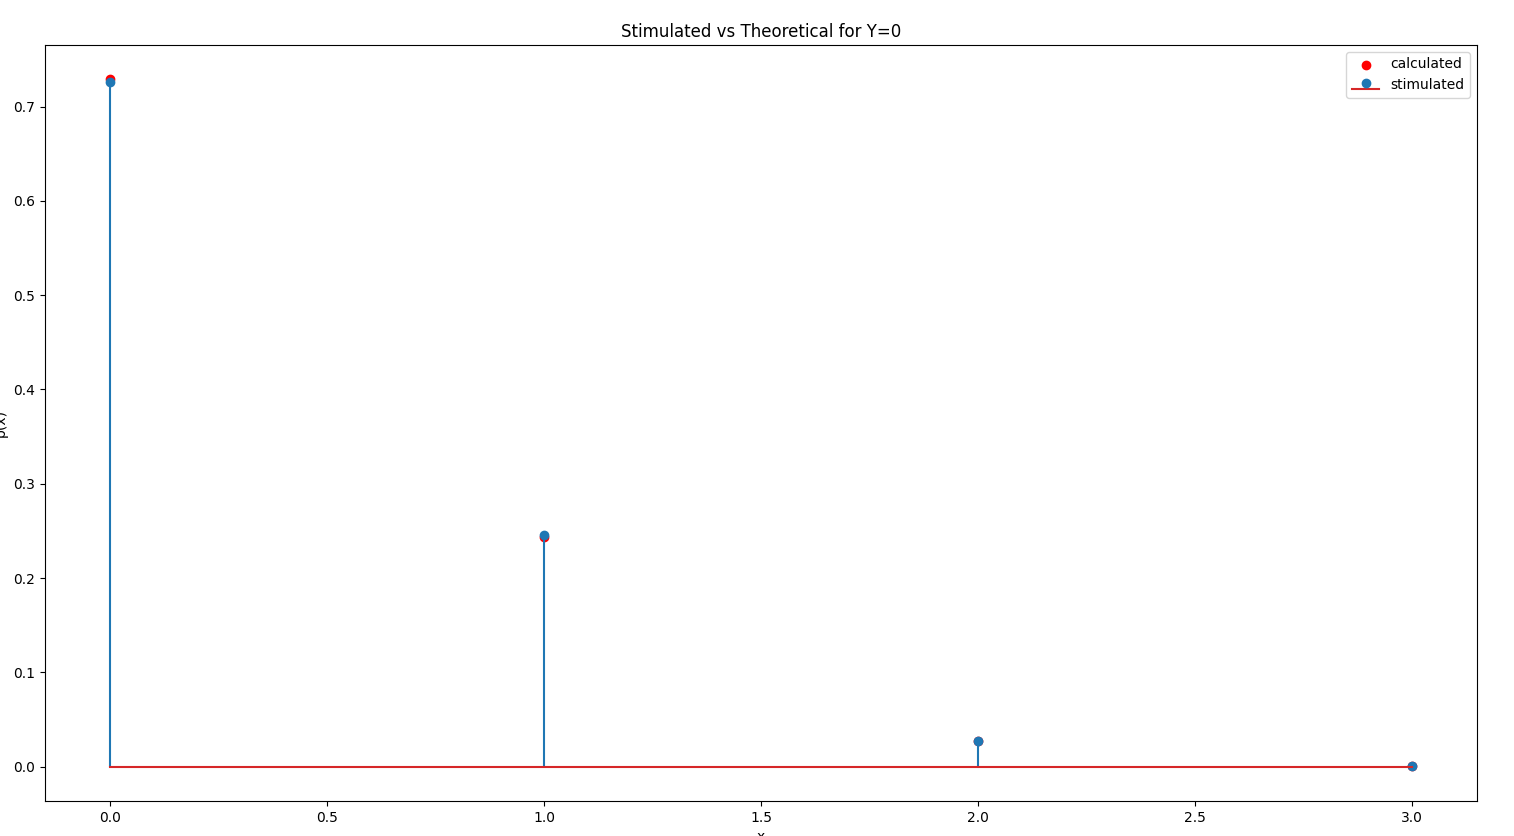
\includegraphics[width=8cm, height=8cm]{assignment2_plot1}
\label{fig:1}
\caption{graph for Y = 0}
\end{figure}
\begin{figure}[H]
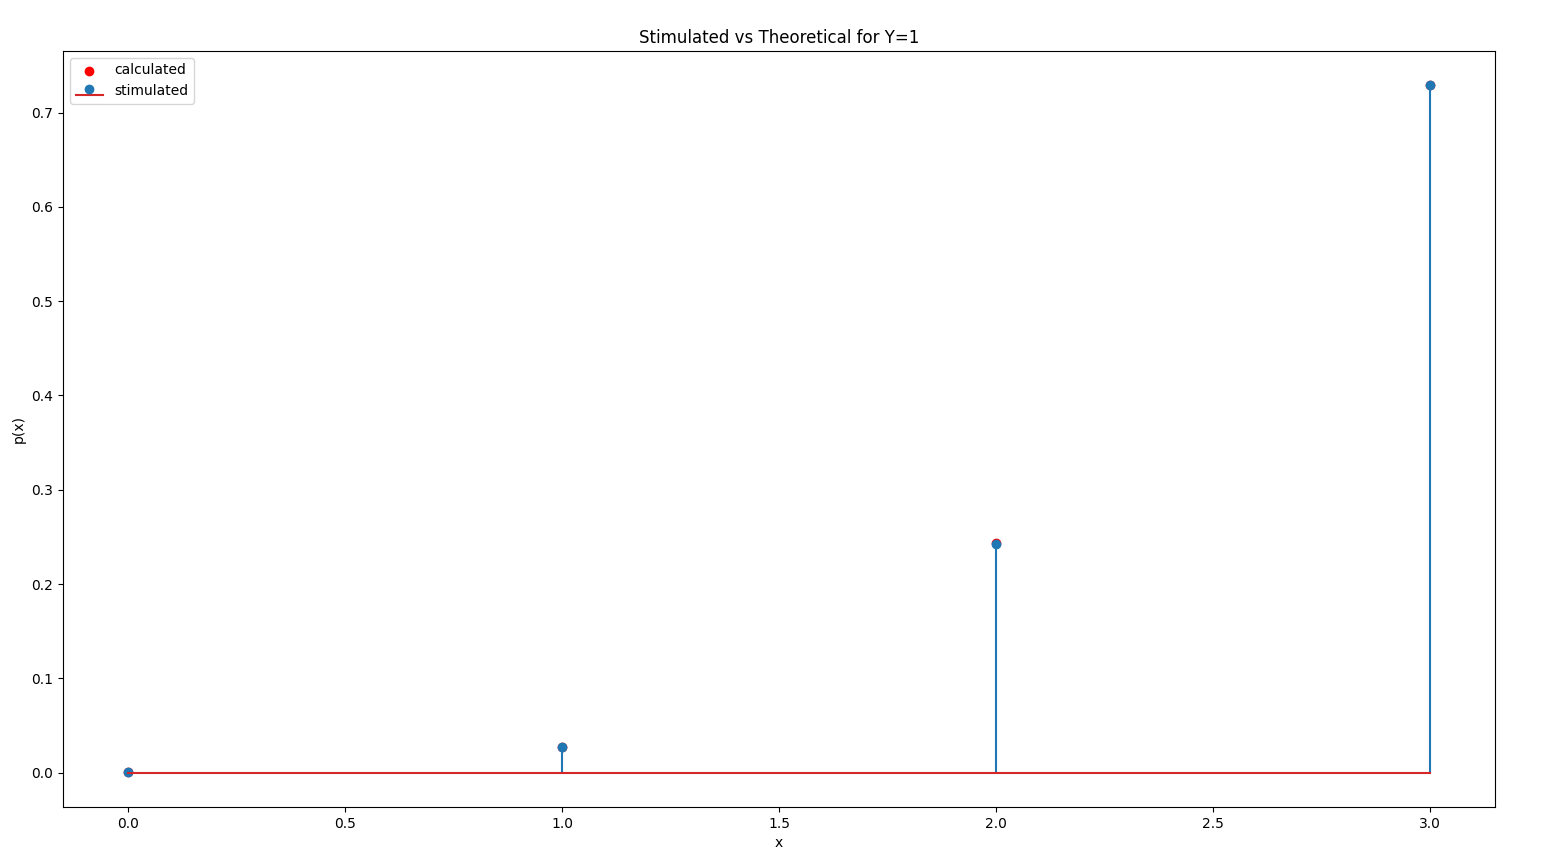
\includegraphics[width=8cm, height=8cm]{assignment2_plot2}
\label{fig:1}
\caption{graph for Y = 1}
\end{figure}
\end{document}